%!TEX root = ../08-Interference.tex
\chapter{Newton's Rings}

The curvature radius of a biconvex lens and the refractive index of water are determined by analyzing the lense's Newton's rings interference pattern.

\section{Setup}

\begin{figure}
	\centering
	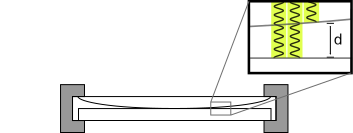
\includegraphics[width=.6\textwidth]{img/newtons-rings.pdf}
	\caption{Newton's rings}
	\caption*{based on \url{https://en.wikipedia.org/wiki/Newton\%27s_rings\#/media/File:Newton\%27s_rings_02.svg}}
\end{figure}

\section{Evaluation}
